% Options for packages loaded elsewhere
\PassOptionsToPackage{unicode}{hyperref}
\PassOptionsToPackage{hyphens}{url}
%
\documentclass[
]{article}
\usepackage{amsmath,amssymb}
\usepackage{iftex}
\ifPDFTeX
  \usepackage[T1]{fontenc}
  \usepackage[utf8]{inputenc}
  \usepackage{textcomp} % provide euro and other symbols
\else % if luatex or xetex
  \usepackage{unicode-math} % this also loads fontspec
  \defaultfontfeatures{Scale=MatchLowercase}
  \defaultfontfeatures[\rmfamily]{Ligatures=TeX,Scale=1}
\fi
\usepackage{lmodern}
\ifPDFTeX\else
  % xetex/luatex font selection
\fi
% Use upquote if available, for straight quotes in verbatim environments
\IfFileExists{upquote.sty}{\usepackage{upquote}}{}
\IfFileExists{microtype.sty}{% use microtype if available
  \usepackage[]{microtype}
  \UseMicrotypeSet[protrusion]{basicmath} % disable protrusion for tt fonts
}{}
\makeatletter
\@ifundefined{KOMAClassName}{% if non-KOMA class
  \IfFileExists{parskip.sty}{%
    \usepackage{parskip}
  }{% else
    \setlength{\parindent}{0pt}
    \setlength{\parskip}{6pt plus 2pt minus 1pt}}
}{% if KOMA class
  \KOMAoptions{parskip=half}}
\makeatother
\usepackage{xcolor}
\usepackage[margin=1in]{geometry}
\usepackage{color}
\usepackage{fancyvrb}
\newcommand{\VerbBar}{|}
\newcommand{\VERB}{\Verb[commandchars=\\\{\}]}
\DefineVerbatimEnvironment{Highlighting}{Verbatim}{commandchars=\\\{\}}
% Add ',fontsize=\small' for more characters per line
\usepackage{framed}
\definecolor{shadecolor}{RGB}{248,248,248}
\newenvironment{Shaded}{\begin{snugshade}}{\end{snugshade}}
\newcommand{\AlertTok}[1]{\textcolor[rgb]{0.94,0.16,0.16}{#1}}
\newcommand{\AnnotationTok}[1]{\textcolor[rgb]{0.56,0.35,0.01}{\textbf{\textit{#1}}}}
\newcommand{\AttributeTok}[1]{\textcolor[rgb]{0.13,0.29,0.53}{#1}}
\newcommand{\BaseNTok}[1]{\textcolor[rgb]{0.00,0.00,0.81}{#1}}
\newcommand{\BuiltInTok}[1]{#1}
\newcommand{\CharTok}[1]{\textcolor[rgb]{0.31,0.60,0.02}{#1}}
\newcommand{\CommentTok}[1]{\textcolor[rgb]{0.56,0.35,0.01}{\textit{#1}}}
\newcommand{\CommentVarTok}[1]{\textcolor[rgb]{0.56,0.35,0.01}{\textbf{\textit{#1}}}}
\newcommand{\ConstantTok}[1]{\textcolor[rgb]{0.56,0.35,0.01}{#1}}
\newcommand{\ControlFlowTok}[1]{\textcolor[rgb]{0.13,0.29,0.53}{\textbf{#1}}}
\newcommand{\DataTypeTok}[1]{\textcolor[rgb]{0.13,0.29,0.53}{#1}}
\newcommand{\DecValTok}[1]{\textcolor[rgb]{0.00,0.00,0.81}{#1}}
\newcommand{\DocumentationTok}[1]{\textcolor[rgb]{0.56,0.35,0.01}{\textbf{\textit{#1}}}}
\newcommand{\ErrorTok}[1]{\textcolor[rgb]{0.64,0.00,0.00}{\textbf{#1}}}
\newcommand{\ExtensionTok}[1]{#1}
\newcommand{\FloatTok}[1]{\textcolor[rgb]{0.00,0.00,0.81}{#1}}
\newcommand{\FunctionTok}[1]{\textcolor[rgb]{0.13,0.29,0.53}{\textbf{#1}}}
\newcommand{\ImportTok}[1]{#1}
\newcommand{\InformationTok}[1]{\textcolor[rgb]{0.56,0.35,0.01}{\textbf{\textit{#1}}}}
\newcommand{\KeywordTok}[1]{\textcolor[rgb]{0.13,0.29,0.53}{\textbf{#1}}}
\newcommand{\NormalTok}[1]{#1}
\newcommand{\OperatorTok}[1]{\textcolor[rgb]{0.81,0.36,0.00}{\textbf{#1}}}
\newcommand{\OtherTok}[1]{\textcolor[rgb]{0.56,0.35,0.01}{#1}}
\newcommand{\PreprocessorTok}[1]{\textcolor[rgb]{0.56,0.35,0.01}{\textit{#1}}}
\newcommand{\RegionMarkerTok}[1]{#1}
\newcommand{\SpecialCharTok}[1]{\textcolor[rgb]{0.81,0.36,0.00}{\textbf{#1}}}
\newcommand{\SpecialStringTok}[1]{\textcolor[rgb]{0.31,0.60,0.02}{#1}}
\newcommand{\StringTok}[1]{\textcolor[rgb]{0.31,0.60,0.02}{#1}}
\newcommand{\VariableTok}[1]{\textcolor[rgb]{0.00,0.00,0.00}{#1}}
\newcommand{\VerbatimStringTok}[1]{\textcolor[rgb]{0.31,0.60,0.02}{#1}}
\newcommand{\WarningTok}[1]{\textcolor[rgb]{0.56,0.35,0.01}{\textbf{\textit{#1}}}}
\usepackage{longtable,booktabs,array}
\usepackage{calc} % for calculating minipage widths
% Correct order of tables after \paragraph or \subparagraph
\usepackage{etoolbox}
\makeatletter
\patchcmd\longtable{\par}{\if@noskipsec\mbox{}\fi\par}{}{}
\makeatother
% Allow footnotes in longtable head/foot
\IfFileExists{footnotehyper.sty}{\usepackage{footnotehyper}}{\usepackage{footnote}}
\makesavenoteenv{longtable}
\usepackage{graphicx}
\makeatletter
\def\maxwidth{\ifdim\Gin@nat@width>\linewidth\linewidth\else\Gin@nat@width\fi}
\def\maxheight{\ifdim\Gin@nat@height>\textheight\textheight\else\Gin@nat@height\fi}
\makeatother
% Scale images if necessary, so that they will not overflow the page
% margins by default, and it is still possible to overwrite the defaults
% using explicit options in \includegraphics[width, height, ...]{}
\setkeys{Gin}{width=\maxwidth,height=\maxheight,keepaspectratio}
% Set default figure placement to htbp
\makeatletter
\def\fps@figure{htbp}
\makeatother
\setlength{\emergencystretch}{3em} % prevent overfull lines
\providecommand{\tightlist}{%
  \setlength{\itemsep}{0pt}\setlength{\parskip}{0pt}}
\setcounter{secnumdepth}{5}
\usepackage{fvextra}
\fvset{breaklines=true, breakanywhere=true}
\ifLuaTeX
  \usepackage{selnolig}  % disable illegal ligatures
\fi
\usepackage{bookmark}
\IfFileExists{xurl.sty}{\usepackage{xurl}}{} % add URL line breaks if available
\urlstyle{same}
\hypersetup{
  pdftitle={PRÁCTICA 2 - Análisis exploratorio de datos},
  pdfauthor={María Victoria León Parra},
  hidelinks,
  pdfcreator={LaTeX via pandoc}}

\title{PRÁCTICA 2 - Análisis exploratorio de datos}
\author{María Victoria León Parra}
\date{2025-05-04}

\begin{document}
\maketitle

{
\setcounter{tocdepth}{2}
\tableofcontents
}
\newpage

\section{Introducción}\label{introducciuxf3n}

Este informe documenta el análisis exploratorio realizado sobre el
conjunto de datos \texttt{massachusetts.csv}, que contiene información
socioeconómica, demográfica y de salud para distintos condados del
estado.

El objetivo principal es familiarizarse con técnicas básicas de
limpieza, exploración y visualización de datos. A lo largo del informe
se realiza:

\begin{itemize}
\tightlist
\item
  La preparación inicial del conjunto de datos, incluyendo limpieza de
  nombres y tratamiento de valores perdidos.
\item
  La creación de variables derivadas útiles para el análisis.
\item
  La identificación de outliers mediante técnicas gráficas y
  estadísticas.
\item
  La generación de visualizaciones para comprender patrones y relaciones
  entre variables.
\item
  Una síntesis de conclusiones basada en los hallazgos obtenidos.
\end{itemize}

\newpage

\section{Carga y preparación de los
datos}\label{carga-y-preparaciuxf3n-de-los-datos}

En esta sección se carga el conjunto de datos original, se realiza una
limpieza básica de los nombres de variables y se explora su estructura.

\begin{Shaded}
\begin{Highlighting}[]
\NormalTok{datos }\OtherTok{\textless{}{-}} \FunctionTok{read\_csv}\NormalTok{(}\StringTok{"../datos/massachusetts.csv"}\NormalTok{) }\SpecialCharTok{|\textgreater{}} 
  \FunctionTok{clean\_names}\NormalTok{()}

\FunctionTok{head}\NormalTok{(datos)}
\end{Highlighting}
\end{Shaded}

\begin{verbatim}
## # A tibble: 6 x 30
##   name           fips  temp   alt   male female    pop suicides firearm_suicides
##   <chr>         <dbl> <dbl> <dbl>  <dbl>  <dbl>  <dbl>    <dbl>            <dbl>
## 1 hampshire co~ 25015  46.3 284.   75022  85808 160830    13.3             3.76 
## 2 suffolk coun~ 25025  51    15.8 388110 415797 803907    43.2             7.05 
## 3 barnstable c~ 25001  50.4  15.6 101791 111199 212990    26.4             6.14 
## 4 worcester co~ 25027  46.9 215.  409610 421012 830622    69.0            18.3  
## 5 nantucket co~ 25019  50    13.7   5856   5543  11399     1.29           NA    
## 6 dukes county  25007  50.6  21.2   8545   8787  17332     1.71            0.571
## # i 21 more variables: homicides <dbl>, vehicle_deaths <dbl>,
## #   labor_force <dbl>, employed <dbl>, unemployed <dbl>, life_expectancy <dbl>,
## #   avg_income <dbl>, less_highschool <dbl>, plus_bachelors <dbl>,
## #   poverty_rate <dbl>, medical_costs <dbl>, food_costs <dbl>,
## #   housing_costs <dbl>, tax_costs <dbl>, poor_health <dbl>, smokers <dbl>,
## #   adult_obesity <dbl>, housing_problems <dbl>, children_in_poverty <dbl>,
## #   uninsured <dbl>, excessive_drinking <dbl>
\end{verbatim}

\begin{Shaded}
\begin{Highlighting}[]
\FunctionTok{str}\NormalTok{(datos)}
\end{Highlighting}
\end{Shaded}

\begin{verbatim}
## spc_tbl_ [14 x 30] (S3: spec_tbl_df/tbl_df/tbl/data.frame)
##  $ name               : chr [1:14] "hampshire county" "suffolk county" "barnstable county" "worcester county" ...
##  $ fips               : num [1:14] 25015 25025 25001 25027 25019 ...
##  $ temp               : num [1:14] 46.3 51 50.4 46.9 50 50.6 47.3 45.6 50.3 49.1 ...
##  $ alt                : num [1:14] 284.3 15.8 15.6 215.2 13.7 ...
##  $ male               : num [1:14] 75022 388110 101791 409610 5856 ...
##  $ female             : num [1:14] 85808 415797 111199 421012 5543 ...
##  $ pop                : num [1:14] 160830 803907 212990 830622 11399 ...
##  $ suicides           : num [1:14] 13.33 43.19 26.38 68.95 1.29 ...
##  $ firearm_suicides   : num [1:14] 3.76 7.05 6.14 18.33 NA ...
##  $ homicides          : num [1:14] 1.05 54.05 2.43 13.67 NA ...
##  $ vehicle_deaths     : num [1:14] 10.2 34.8 21.9 65.6 NA ...
##  $ labor_force        : num [1:14] 85661 446558 108128 432005 7664 ...
##  $ employed           : num [1:14] 79477 403388 97073 394081 6873 ...
##  $ unemployed         : num [1:14] 6184 43170 11055 37924 791 ...
##  $ life_expectancy    : num [1:14] 80.8 79.9 80.8 79.7 81.6 ...
##  $ avg_income         : num [1:14] 52984 81152 74756 57003 124168 ...
##  $ less_highschool    : num [1:14] 5.3 13.7 4.5 9.3 4.4 5.2 14.2 8.7 14.3 6.6 ...
##  $ plus_bachelors     : num [1:14] 48.3 46.1 43.4 36.4 52.8 44.9 27.1 33.6 28.7 56.3 ...
##  $ poverty_rate       : num [1:14] 11.1 16.7 6.5 9.4 5.5 7.3 13.8 11.2 11.3 6.9 ...
##  $ medical_costs      : num [1:14] 3048 3048 3048 3048 3048 ...
##  $ food_costs         : num [1:14] 3690 3690 3690 3690 3690 3690 3690 3690 3690 3690 ...
##  $ housing_costs      : num [1:14] 8844 20580 11832 11052 14976 ...
##  $ tax_costs          : num [1:14] 4003 5906 4488 4361 4997 ...
##  $ poor_health        : num [1:14] 13.6 17.8 12.7 14.7 12 ...
##  $ smokers            : num [1:14] 16.1 15.8 16.1 17.6 13.2 ...
##  $ adult_obesity      : num [1:14] 21.4 21.4 22.5 28.3 25.1 28.4 30.5 26.7 28.7 21.6 ...
##  $ housing_problems   : num [1:14] 16.4 24.5 17.1 15.9 19.9 ...
##  $ children_in_poverty: num [1:14] 9.9 23.9 10.1 11.9 5.8 11.6 20.2 16.3 16 7.1 ...
##  $ uninsured          : num [1:14] 2.83 4.41 3.75 3.08 4.45 ...
##  $ excessive_drinking : num [1:14] 22.5 23 26.5 22.1 23.6 ...
##  - attr(*, "spec")=
##   .. cols(
##   ..   name = col_character(),
##   ..   fips = col_double(),
##   ..   temp = col_double(),
##   ..   alt = col_double(),
##   ..   male = col_double(),
##   ..   female = col_double(),
##   ..   pop = col_double(),
##   ..   suicides = col_double(),
##   ..   firearm_suicides = col_double(),
##   ..   homicides = col_double(),
##   ..   vehicle_deaths = col_double(),
##   ..   labor_force = col_double(),
##   ..   employed = col_double(),
##   ..   unemployed = col_double(),
##   ..   life_expectancy = col_double(),
##   ..   avg_income = col_double(),
##   ..   less_highschool = col_double(),
##   ..   plus_bachelors = col_double(),
##   ..   poverty_rate = col_double(),
##   ..   medical_costs = col_double(),
##   ..   food_costs = col_double(),
##   ..   housing_costs = col_double(),
##   ..   tax_costs = col_double(),
##   ..   poor_health = col_double(),
##   ..   smokers = col_double(),
##   ..   adult_obesity = col_double(),
##   ..   housing_problems = col_double(),
##   ..   children_in_poverty = col_double(),
##   ..   uninsured = col_double(),
##   ..   excessive_drinking = col_double()
##   .. )
##  - attr(*, "problems")=<externalptr>
\end{verbatim}

\begin{Shaded}
\begin{Highlighting}[]
\FunctionTok{skim}\NormalTok{(datos)}
\end{Highlighting}
\end{Shaded}

\begin{longtable}[]{@{}ll@{}}
\caption{Data summary}\tabularnewline
\toprule\noalign{}
\endfirsthead
\endhead
\bottomrule\noalign{}
\endlastfoot
Name & datos \\
Number of rows & 14 \\
Number of columns & 30 \\
\_\_\_\_\_\_\_\_\_\_\_\_\_\_\_\_\_\_\_\_\_\_\_ & \\
Column type frequency: & \\
character & 1 \\
numeric & 29 \\
\_\_\_\_\_\_\_\_\_\_\_\_\_\_\_\_\_\_\_\_\_\_\_\_ & \\
Group variables & None \\
\end{longtable}

\textbf{Variable type: character}

\begin{longtable}[]{@{}
  >{\raggedright\arraybackslash}p{(\columnwidth - 14\tabcolsep) * \real{0.1944}}
  >{\raggedleft\arraybackslash}p{(\columnwidth - 14\tabcolsep) * \real{0.1389}}
  >{\raggedleft\arraybackslash}p{(\columnwidth - 14\tabcolsep) * \real{0.1944}}
  >{\raggedleft\arraybackslash}p{(\columnwidth - 14\tabcolsep) * \real{0.0556}}
  >{\raggedleft\arraybackslash}p{(\columnwidth - 14\tabcolsep) * \real{0.0556}}
  >{\raggedleft\arraybackslash}p{(\columnwidth - 14\tabcolsep) * \real{0.0833}}
  >{\raggedleft\arraybackslash}p{(\columnwidth - 14\tabcolsep) * \real{0.1250}}
  >{\raggedleft\arraybackslash}p{(\columnwidth - 14\tabcolsep) * \real{0.1528}}@{}}
\toprule\noalign{}
\begin{minipage}[b]{\linewidth}\raggedright
skim\_variable
\end{minipage} & \begin{minipage}[b]{\linewidth}\raggedleft
n\_missing
\end{minipage} & \begin{minipage}[b]{\linewidth}\raggedleft
complete\_rate
\end{minipage} & \begin{minipage}[b]{\linewidth}\raggedleft
min
\end{minipage} & \begin{minipage}[b]{\linewidth}\raggedleft
max
\end{minipage} & \begin{minipage}[b]{\linewidth}\raggedleft
empty
\end{minipage} & \begin{minipage}[b]{\linewidth}\raggedleft
n\_unique
\end{minipage} & \begin{minipage}[b]{\linewidth}\raggedleft
whitespace
\end{minipage} \\
\midrule\noalign{}
\endhead
\bottomrule\noalign{}
\endlastfoot
name & 0 & 1 & 12 & 17 & 0 & 14 & 0 \\
\end{longtable}

\textbf{Variable type: numeric}

\begin{longtable}[]{@{}
  >{\raggedright\arraybackslash}p{(\columnwidth - 20\tabcolsep) * \real{0.1667}}
  >{\raggedleft\arraybackslash}p{(\columnwidth - 20\tabcolsep) * \real{0.0833}}
  >{\raggedleft\arraybackslash}p{(\columnwidth - 20\tabcolsep) * \real{0.1167}}
  >{\raggedleft\arraybackslash}p{(\columnwidth - 20\tabcolsep) * \real{0.0833}}
  >{\raggedleft\arraybackslash}p{(\columnwidth - 20\tabcolsep) * \real{0.0833}}
  >{\raggedleft\arraybackslash}p{(\columnwidth - 20\tabcolsep) * \real{0.0750}}
  >{\raggedleft\arraybackslash}p{(\columnwidth - 20\tabcolsep) * \real{0.0833}}
  >{\raggedleft\arraybackslash}p{(\columnwidth - 20\tabcolsep) * \real{0.0833}}
  >{\raggedleft\arraybackslash}p{(\columnwidth - 20\tabcolsep) * \real{0.0833}}
  >{\raggedleft\arraybackslash}p{(\columnwidth - 20\tabcolsep) * \real{0.0917}}
  >{\raggedright\arraybackslash}p{(\columnwidth - 20\tabcolsep) * \real{0.0500}}@{}}
\toprule\noalign{}
\begin{minipage}[b]{\linewidth}\raggedright
skim\_variable
\end{minipage} & \begin{minipage}[b]{\linewidth}\raggedleft
n\_missing
\end{minipage} & \begin{minipage}[b]{\linewidth}\raggedleft
complete\_rate
\end{minipage} & \begin{minipage}[b]{\linewidth}\raggedleft
mean
\end{minipage} & \begin{minipage}[b]{\linewidth}\raggedleft
sd
\end{minipage} & \begin{minipage}[b]{\linewidth}\raggedleft
p0
\end{minipage} & \begin{minipage}[b]{\linewidth}\raggedleft
p25
\end{minipage} & \begin{minipage}[b]{\linewidth}\raggedleft
p50
\end{minipage} & \begin{minipage}[b]{\linewidth}\raggedleft
p75
\end{minipage} & \begin{minipage}[b]{\linewidth}\raggedleft
p100
\end{minipage} & \begin{minipage}[b]{\linewidth}\raggedright
hist
\end{minipage} \\
\midrule\noalign{}
\endhead
\bottomrule\noalign{}
\endlastfoot
fips & 0 & 1.00 & 25014.00 & 8.37 & 25001.00 & 25007.50 & 25014.00 &
25020.50 & 25027.00 & ▇▇▅▇▇ \\
temp & 0 & 1.00 & 48.71 & 1.92 & 45.60 & 47.00 & 49.25 & 50.25 & 51.00 &
▃▂▁▃▇ \\
alt & 0 & 1.00 & 104.26 & 116.20 & 13.70 & 22.00 & 37.65 & 193.33 &
354.10 & ▇▁▂▁▁ \\
male & 0 & 1.00 & 238969.14 & 217198.62 & 5856.00 & 64060.00 & 239246.50
& 370313.25 & 789545.00 & ▇▃▅▁▁ \\
female & 0 & 1.00 & 253352.50 & 226885.69 & 5543.00 & 69855.50 &
254540.50 & 398156.00 & 822154.00 & ▇▃▅▁▁ \\
pop & 0 & 1.00 & 492321.64 & 444052.35 & 11399.00 & 133915.50 &
493787.00 & 768469.25 & 1611699.00 & ▇▃▅▁▁ \\
suicides & 0 & 1.00 & 38.46 & 30.65 & 1.29 & 13.69 & 43.40 & 50.71 &
111.71 & ▇▆▅▂▂ \\
firearm\_suicides & 1 & 0.93 & 9.22 & 5.90 & 0.57 & 4.52 & 8.81 & 13.00
& 19.67 & ▇▇▇▅▅ \\
homicides & 2 & 0.86 & 13.25 & 14.55 & 0.67 & 2.40 & 12.38 & 15.42 &
54.05 & ▇▇▁▁▁ \\
vehicle\_deaths & 1 & 0.93 & 35.30 & 23.00 & 1.29 & 15.48 & 40.10 &
46.95 & 75.14 & ▇▂▇▃▃ \\
labor\_force & 0 & 1.00 & 261308.71 & 241931.63 & 7664.00 & 67649.00 &
248496.00 & 406010.25 & 882398.00 & ▇▃▅▁▁ \\
employed & 0 & 1.00 & 238152.00 & 222953.50 & 6873.00 & 61881.25 &
223975.50 & 367638.25 & 818205.00 & ▇▃▅▁▁ \\
unemployed & 0 & 1.00 & 23156.71 & 19382.87 & 791.00 & 5767.75 &
24520.50 & 36376.25 & 64193.00 & ▇▁▅▂▁ \\
life\_expectancy & 0 & 1.00 & 80.45 & 0.97 & 78.85 & 79.72 & 80.39 &
81.22 & 82.05 & ▃▇▇▂▆ \\
avg\_income & 0 & 1.00 & 72239.21 & 21040.98 & 51187.00 & 55142.50 &
67506.00 & 83134.25 & 124168.00 & ▇▃▅▁▁ \\
less\_highschool & 0 & 1.00 & 8.34 & 3.58 & 4.40 & 5.50 & 6.90 & 10.35 &
14.30 & ▇▅▃▂▅ \\
plus\_bachelors & 0 & 1.00 & 41.86 & 9.07 & 27.10 & 36.62 & 41.65 &
47.75 & 56.30 & ▃▇▃▆▆ \\
poverty\_rate & 0 & 1.00 & 9.36 & 3.21 & 5.50 & 7.00 & 9.05 & 11.17 &
16.70 & ▇▃▃▁▁ \\
medical\_costs & 0 & 1.00 & 3048.00 & 0.00 & 3048.00 & 3048.00 & 3048.00
& 3048.00 & 3048.00 & ▁▁▇▁▁ \\
food\_costs & 0 & 1.00 & 3690.00 & 0.00 & 3690.00 & 3690.00 & 3690.00 &
3690.00 & 3690.00 & ▁▁▇▁▁ \\
housing\_costs & 0 & 1.00 & 13795.57 & 4386.15 & 8844.00 & 9885.75 &
12672.00 & 17595.50 & 20580.00 & ▇▂▁▂▃ \\
tax\_costs & 0 & 1.00 & 4805.86 & 711.15 & 4003.00 & 4171.75 & 4624.00 &
5421.50 & 5906.00 & ▇▂▁▂▃ \\
poor\_health & 0 & 1.00 & 14.24 & 2.31 & 11.12 & 12.53 & 14.23 & 15.04 &
19.07 & ▇▃▆▂▃ \\
smokers & 0 & 1.00 & 16.15 & 2.21 & 12.33 & 15.05 & 16.11 & 18.06 &
19.48 & ▅▂▇▂▆ \\
adult\_obesity & 0 & 1.00 & 25.79 & 3.07 & 21.40 & 23.02 & 26.40 & 28.37
& 30.50 & ▇▂▆▇▃ \\
housing\_problems & 0 & 1.00 & 17.85 & 3.18 & 14.66 & 15.88 & 16.62 &
18.83 & 24.47 & ▇▂▃▁▂ \\
children\_in\_poverty & 0 & 1.00 & 12.21 & 5.29 & 5.50 & 9.45 & 11.55 &
14.97 & 23.90 & ▃▇▂▁▁ \\
uninsured & 0 & 1.00 & 3.44 & 0.64 & 2.38 & 2.89 & 3.59 & 3.81 & 4.45 &
▅▅▂▇▃ \\
excessive\_drinking & 0 & 1.00 & 23.95 & 1.55 & 22.08 & 22.79 & 23.40 &
25.44 & 26.45 & ▇▇▂▂▇ \\
\end{longtable}

\newpage

\section{Tratamiento de valores
faltantes}\label{tratamiento-de-valores-faltantes}

Se identifican y visualizan los valores faltantes. Posteriormente, se
aplican técnicas de imputación para rellenar esos valores con la media
en las variables numéricas.

\begin{Shaded}
\begin{Highlighting}[]
\FunctionTok{gg\_miss\_var}\NormalTok{(datos) }\SpecialCharTok{+}
  \FunctionTok{labs}\NormalTok{(}\AttributeTok{title =} \StringTok{"Valores NA por variable"}\NormalTok{, }\AttributeTok{x =} \StringTok{"Variables"}\NormalTok{, }\AttributeTok{y =} \StringTok{"Número de valores NA"}\NormalTok{)}
\end{Highlighting}
\end{Shaded}

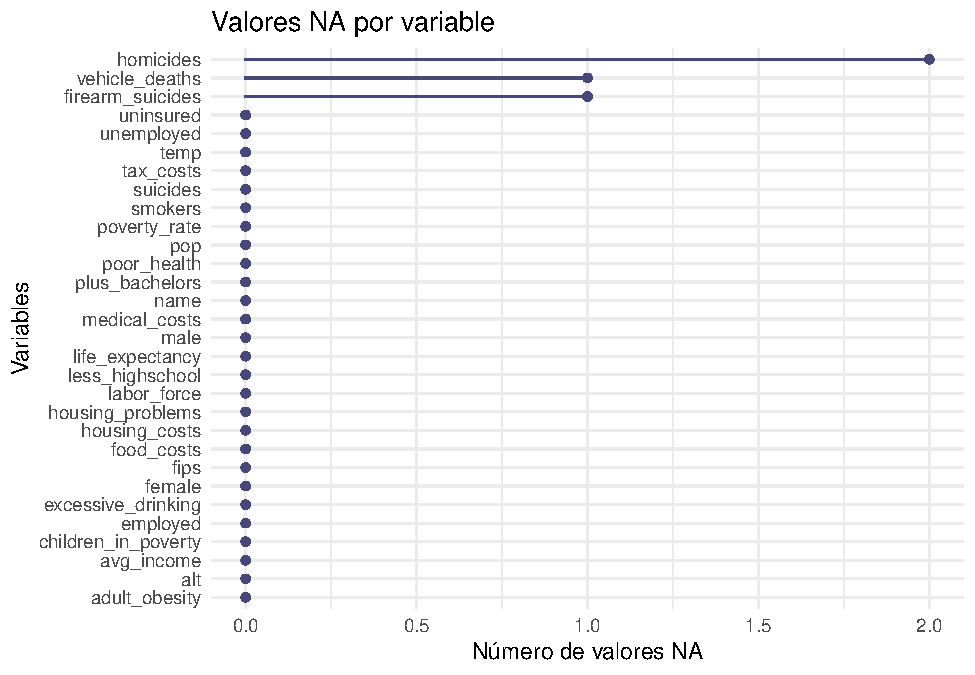
\includegraphics{Informe_P2_files/figure-latex/valores-faltantes-1.pdf}

\begin{Shaded}
\begin{Highlighting}[]
\FunctionTok{ggsave}\NormalTok{(}\StringTok{"../salida/na\_por\_variable.png"}\NormalTok{, }\AttributeTok{width =} \DecValTok{8}\NormalTok{, }\AttributeTok{height =} \DecValTok{5}\NormalTok{, }\AttributeTok{bg =} \StringTok{"white"}\NormalTok{)}
\end{Highlighting}
\end{Shaded}

\begin{Shaded}
\begin{Highlighting}[]
\NormalTok{datos }\OtherTok{\textless{}{-}}\NormalTok{ datos }\SpecialCharTok{|\textgreater{}} 
  \FunctionTok{mutate}\NormalTok{(}\FunctionTok{across}\NormalTok{(}\FunctionTok{where}\NormalTok{(is.numeric), }\SpecialCharTok{\textasciitilde{}}\FunctionTok{replace\_na}\NormalTok{(., }\FunctionTok{mean}\NormalTok{(., }\AttributeTok{na.rm =} \ConstantTok{TRUE}\NormalTok{))))}
\end{Highlighting}
\end{Shaded}

\newpage

\section{Creación de nuevas
variables}\label{creaciuxf3n-de-nuevas-variables}

Se generan variables derivadas a partir de las existentes que resultan
más informativas para el análisis.

\begin{Shaded}
\begin{Highlighting}[]
\NormalTok{datos }\OtherTok{\textless{}{-}}\NormalTok{ datos }\SpecialCharTok{|\textgreater{}} 
  \FunctionTok{mutate}\NormalTok{(}
    \AttributeTok{prop\_hombres =}\NormalTok{ male }\SpecialCharTok{/}\NormalTok{ pop,}
    \AttributeTok{prop\_mujeres =}\NormalTok{ female }\SpecialCharTok{/}\NormalTok{ pop,}
    \AttributeTok{tasa\_paro =}\NormalTok{ unemployed }\SpecialCharTok{/}\NormalTok{ labor\_force,}
    \AttributeTok{tasa\_suicidios =}\NormalTok{ suicides }\SpecialCharTok{/}\NormalTok{ pop }\SpecialCharTok{*} \DecValTok{100000}\NormalTok{,}
    \AttributeTok{tasa\_homicidios =}\NormalTok{ homicides }\SpecialCharTok{/}\NormalTok{ pop }\SpecialCharTok{*} \DecValTok{100000}
\NormalTok{  )}
\end{Highlighting}
\end{Shaded}

\newpage

\section{Identificación de
outliers}\label{identificaciuxf3n-de-outliers}

Aquí se detectan valores atípicos. Además, se consolida una tabla con
los condados que presentan outliers en distintas variables clave.

\begin{Shaded}
\begin{Highlighting}[]
\FunctionTok{ggplot}\NormalTok{(datos, }\FunctionTok{aes}\NormalTok{(}\AttributeTok{y =}\NormalTok{ suicides)) }\SpecialCharTok{+}
  \FunctionTok{geom\_boxplot}\NormalTok{(}\AttributeTok{fill =} \StringTok{"lightblue"}\NormalTok{, }\AttributeTok{outlier.color =} \StringTok{"red"}\NormalTok{) }\SpecialCharTok{+}
  \FunctionTok{labs}\NormalTok{(}\AttributeTok{title =} \StringTok{"Outliers en la variable \textquotesingle{}suicides\textquotesingle{}"}\NormalTok{, }\AttributeTok{y =} \StringTok{"Tasa de suicidios"}\NormalTok{) }\SpecialCharTok{+}
  \FunctionTok{theme\_minimal}\NormalTok{()}
\end{Highlighting}
\end{Shaded}

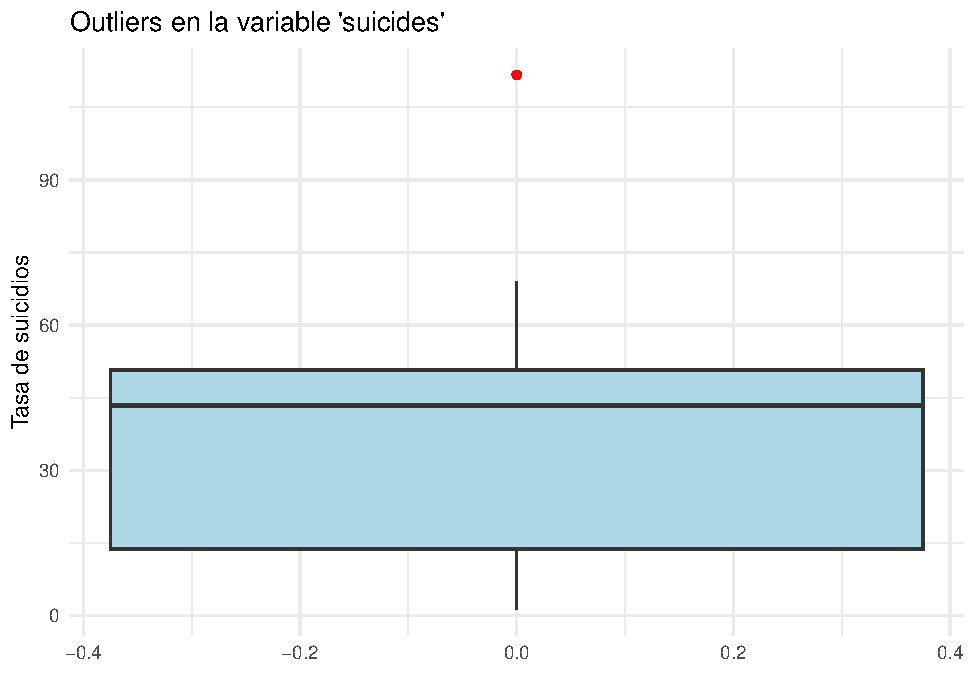
\includegraphics{Informe_P2_files/figure-latex/boxplot-suicides-1.pdf}

\begin{Shaded}
\begin{Highlighting}[]
\FunctionTok{ggsave}\NormalTok{(}\StringTok{"../salida/boxplot\_suicides.png"}\NormalTok{, }\AttributeTok{width =} \DecValTok{6}\NormalTok{, }\AttributeTok{height =} \DecValTok{5}\NormalTok{, }\AttributeTok{bg =} \StringTok{"white"}\NormalTok{)}
\end{Highlighting}
\end{Shaded}

\begin{Shaded}
\begin{Highlighting}[]
\NormalTok{outliers\_suicides }\OtherTok{\textless{}{-}} \FunctionTok{boxplot.stats}\NormalTok{(datos}\SpecialCharTok{$}\NormalTok{suicides)}\SpecialCharTok{$}\NormalTok{out}
\NormalTok{outliers\_tabla }\OtherTok{\textless{}{-}}\NormalTok{ datos }\SpecialCharTok{|\textgreater{}} \FunctionTok{filter}\NormalTok{(suicides }\SpecialCharTok{\%in\%}\NormalTok{ outliers\_suicides) }\SpecialCharTok{|\textgreater{}} \FunctionTok{select}\NormalTok{(name, suicides)}

\NormalTok{outliers\_por\_variable }\OtherTok{\textless{}{-}} \FunctionTok{list}\NormalTok{()}
\NormalTok{numeric\_vars }\OtherTok{\textless{}{-}}\NormalTok{ datos }\SpecialCharTok{|\textgreater{}} \FunctionTok{select}\NormalTok{(}\FunctionTok{where}\NormalTok{(is.numeric), }\SpecialCharTok{{-}}\NormalTok{fips) }\SpecialCharTok{|\textgreater{}} \FunctionTok{names}\NormalTok{()}

\ControlFlowTok{for}\NormalTok{ (var }\ControlFlowTok{in}\NormalTok{ numeric\_vars) \{}
\NormalTok{  valores\_out }\OtherTok{\textless{}{-}} \FunctionTok{boxplot.stats}\NormalTok{(datos[[var]])}\SpecialCharTok{$}\NormalTok{out}
  \ControlFlowTok{if}\NormalTok{ (}\FunctionTok{length}\NormalTok{(valores\_out) }\SpecialCharTok{\textgreater{}} \DecValTok{0}\NormalTok{) \{}
\NormalTok{    condados }\OtherTok{\textless{}{-}}\NormalTok{ datos }\SpecialCharTok{|\textgreater{}} \FunctionTok{filter}\NormalTok{(.data[[var]] }\SpecialCharTok{\%in\%}\NormalTok{ valores\_out) }\SpecialCharTok{|\textgreater{}} \FunctionTok{pull}\NormalTok{(name)}
\NormalTok{    outliers\_por\_variable[[var]] }\OtherTok{\textless{}{-}} \FunctionTok{unique}\NormalTok{(condados)}
\NormalTok{  \}}
\NormalTok{\}}

\NormalTok{outliers\_tabla }\OtherTok{\textless{}{-}} \FunctionTok{full\_join}\NormalTok{(outliers\_tabla, datos }\SpecialCharTok{|\textgreater{}} \FunctionTok{filter}\NormalTok{(name }\SpecialCharTok{\%in\%}\NormalTok{ outliers\_por\_variable}\SpecialCharTok{$}\NormalTok{homicides) }\SpecialCharTok{|\textgreater{}} \FunctionTok{select}\NormalTok{(name, homicides), }\AttributeTok{by =} \StringTok{"name"}\NormalTok{)}
\NormalTok{outliers\_tabla }\OtherTok{\textless{}{-}} \FunctionTok{full\_join}\NormalTok{(outliers\_tabla, datos }\SpecialCharTok{|\textgreater{}} \FunctionTok{filter}\NormalTok{(name }\SpecialCharTok{\%in\%}\NormalTok{ outliers\_por\_variable}\SpecialCharTok{$}\NormalTok{housing\_problems) }\SpecialCharTok{|\textgreater{}} \FunctionTok{select}\NormalTok{(name, housing\_problems), }\AttributeTok{by =} \StringTok{"name"}\NormalTok{)}
\NormalTok{outliers\_tabla }\OtherTok{\textless{}{-}} \FunctionTok{full\_join}\NormalTok{(outliers\_tabla, datos }\SpecialCharTok{|\textgreater{}} \FunctionTok{filter}\NormalTok{(name }\SpecialCharTok{\%in\%}\NormalTok{ outliers\_por\_variable}\SpecialCharTok{$}\NormalTok{tasa\_homicidios) }\SpecialCharTok{|\textgreater{}} \FunctionTok{select}\NormalTok{(name, tasa\_homicidios), }\AttributeTok{by =} \StringTok{"name"}\NormalTok{)}
\NormalTok{outliers\_tabla }\OtherTok{\textless{}{-}} \FunctionTok{full\_join}\NormalTok{(outliers\_tabla, datos }\SpecialCharTok{|\textgreater{}} \FunctionTok{filter}\NormalTok{(name }\SpecialCharTok{\%in\%}\NormalTok{ outliers\_por\_variable}\SpecialCharTok{$}\NormalTok{prop\_hombres) }\SpecialCharTok{|\textgreater{}} \FunctionTok{select}\NormalTok{(name, prop\_hombres), }\AttributeTok{by =} \StringTok{"name"}\NormalTok{)}
\NormalTok{outliers\_tabla }\OtherTok{\textless{}{-}} \FunctionTok{full\_join}\NormalTok{(outliers\_tabla, datos }\SpecialCharTok{|\textgreater{}} \FunctionTok{filter}\NormalTok{(name }\SpecialCharTok{\%in\%}\NormalTok{ outliers\_por\_variable}\SpecialCharTok{$}\NormalTok{prop\_mujeres) }\SpecialCharTok{|\textgreater{}} \FunctionTok{select}\NormalTok{(name, prop\_mujeres), }\AttributeTok{by =} \StringTok{"name"}\NormalTok{)}

\FunctionTok{write\_csv}\NormalTok{(outliers\_tabla, }\StringTok{"../salida/outliers\_tabla.csv"}\NormalTok{)}
\end{Highlighting}
\end{Shaded}

\newpage

\section{Estadísticas descriptivas}\label{estaduxedsticas-descriptivas}

Esta sección incluye resúmenes estadísticos de todas las variables,
permitiendo identificar rangos, medias, desviaciones y posibles
anomalías en los datos.

\begin{Shaded}
\begin{Highlighting}[]
\FunctionTok{sink}\NormalTok{(}\StringTok{"../salida/resumen\_summary.txt"}\NormalTok{)}
\FunctionTok{summary}\NormalTok{(}\FunctionTok{select}\NormalTok{(datos, }\SpecialCharTok{{-}}\NormalTok{name))}
\FunctionTok{sink}\NormalTok{()}
\end{Highlighting}
\end{Shaded}

\begin{Shaded}
\begin{Highlighting}[]
\FunctionTok{sink}\NormalTok{(}\StringTok{"../salida/resumen\_skim.txt"}\NormalTok{)}
\FunctionTok{print}\NormalTok{(}\FunctionTok{skim}\NormalTok{(}\FunctionTok{select}\NormalTok{(datos, }\SpecialCharTok{{-}}\NormalTok{name)))}
\FunctionTok{sink}\NormalTok{()}
\end{Highlighting}
\end{Shaded}

\newpage

\section{Visualización de datos}\label{visualizaciuxf3n-de-datos}

Se presentan diversas visualizaciones para explorar la distribución de
variables y relaciones entre ellas.

\subsection{Histograma del ingreso
medio}\label{histograma-del-ingreso-medio}

\begin{Shaded}
\begin{Highlighting}[]
\FunctionTok{ggplot}\NormalTok{(datos, }\FunctionTok{aes}\NormalTok{(}\AttributeTok{x =}\NormalTok{ avg\_income)) }\SpecialCharTok{+}
  \FunctionTok{geom\_histogram}\NormalTok{(}\AttributeTok{binwidth =} \DecValTok{5000}\NormalTok{, }\AttributeTok{fill =} \StringTok{"steelblue"}\NormalTok{, }\AttributeTok{color =} \StringTok{"white"}\NormalTok{) }\SpecialCharTok{+}
  \FunctionTok{geom\_vline}\NormalTok{(}\FunctionTok{aes}\NormalTok{(}\AttributeTok{xintercept =} \FunctionTok{mean}\NormalTok{(avg\_income)), }\AttributeTok{color =} \StringTok{"red"}\NormalTok{, }\AttributeTok{linetype =} \StringTok{"dashed"}\NormalTok{, }\AttributeTok{size =} \DecValTok{1}\NormalTok{) }\SpecialCharTok{+}
  \FunctionTok{labs}\NormalTok{(}\AttributeTok{title =} \StringTok{"Distribución del ingreso medio"}\NormalTok{, }\AttributeTok{x =} \StringTok{"Ingreso medio"}\NormalTok{, }\AttributeTok{y =} \StringTok{"Frecuencia"}\NormalTok{) }\SpecialCharTok{+}
  \FunctionTok{theme\_minimal}\NormalTok{()}
\end{Highlighting}
\end{Shaded}

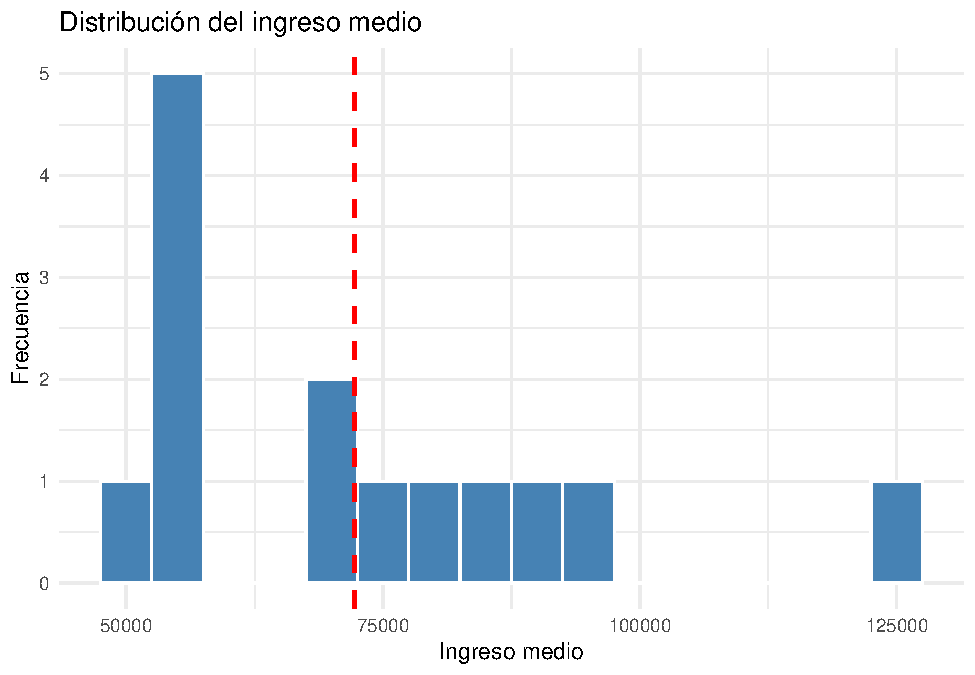
\includegraphics{Informe_P2_files/figure-latex/histograma-1.pdf}

\begin{Shaded}
\begin{Highlighting}[]
\FunctionTok{ggsave}\NormalTok{(}\StringTok{"../salida/histograma\_avg\_income.png"}\NormalTok{, }\AttributeTok{width =} \DecValTok{7}\NormalTok{, }\AttributeTok{height =} \DecValTok{5}\NormalTok{, }\AttributeTok{bg =} \StringTok{"white"}\NormalTok{)}
\end{Highlighting}
\end{Shaded}

\newpage

\subsection{Densidad del ingreso
medio}\label{densidad-del-ingreso-medio}

\begin{Shaded}
\begin{Highlighting}[]
\FunctionTok{ggplot}\NormalTok{(datos, }\FunctionTok{aes}\NormalTok{(}\AttributeTok{x =}\NormalTok{ avg\_income)) }\SpecialCharTok{+}
  \FunctionTok{geom\_density}\NormalTok{(}\AttributeTok{fill =} \StringTok{"skyblue"}\NormalTok{, }\AttributeTok{alpha =} \FloatTok{0.5}\NormalTok{) }\SpecialCharTok{+}
  \FunctionTok{labs}\NormalTok{(}\AttributeTok{title =} \StringTok{"Densidad del ingreso medio"}\NormalTok{, }\AttributeTok{x =} \StringTok{"Ingreso medio"}\NormalTok{, }\AttributeTok{y =} \StringTok{"Densidad"}\NormalTok{) }\SpecialCharTok{+}
  \FunctionTok{theme\_minimal}\NormalTok{()}
\end{Highlighting}
\end{Shaded}

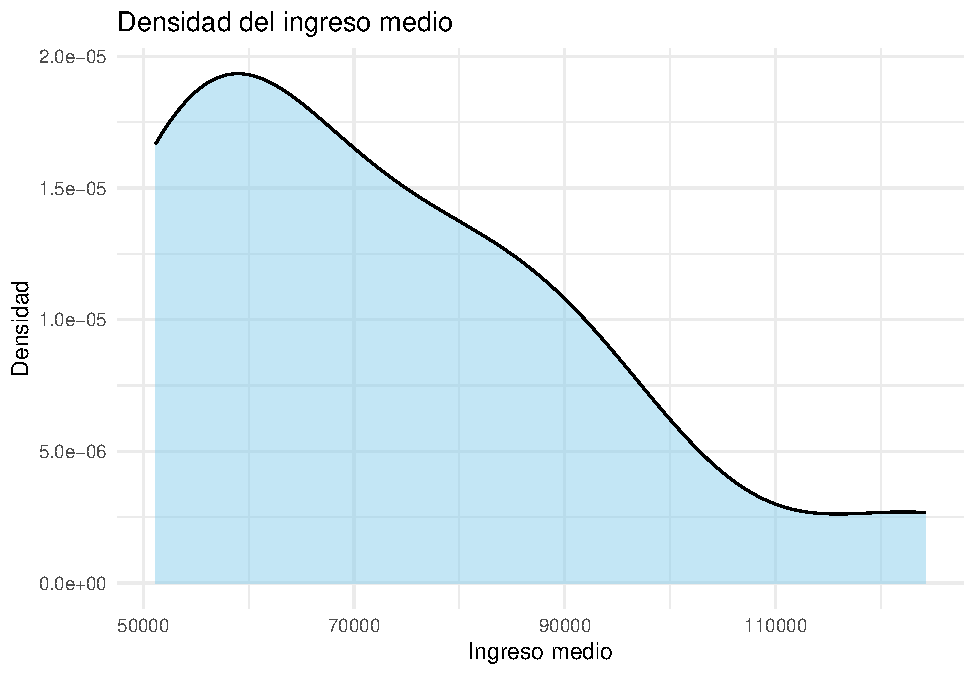
\includegraphics{Informe_P2_files/figure-latex/densidad-1.pdf}

\begin{Shaded}
\begin{Highlighting}[]
\FunctionTok{ggsave}\NormalTok{(}\StringTok{"../salida/densidad\_avg\_income.png"}\NormalTok{, }\AttributeTok{width =} \DecValTok{7}\NormalTok{, }\AttributeTok{height =} \DecValTok{5}\NormalTok{, }\AttributeTok{bg =} \StringTok{"white"}\NormalTok{)}
\end{Highlighting}
\end{Shaded}

\newpage

\subsection{Boxplot de homicidios}\label{boxplot-de-homicidios}

\begin{Shaded}
\begin{Highlighting}[]
\FunctionTok{ggplot}\NormalTok{(datos, }\FunctionTok{aes}\NormalTok{(}\AttributeTok{y =}\NormalTok{ homicides)) }\SpecialCharTok{+}
  \FunctionTok{geom\_boxplot}\NormalTok{(}\AttributeTok{fill =} \StringTok{"cadetblue"}\NormalTok{, }\AttributeTok{outlier.color =} \StringTok{"red"}\NormalTok{) }\SpecialCharTok{+}
  \FunctionTok{labs}\NormalTok{(}\AttributeTok{title =} \StringTok{"Boxplot del número de homicidios por condado"}\NormalTok{, }\AttributeTok{y =} \StringTok{"Número de homicidios"}\NormalTok{) }\SpecialCharTok{+}
  \FunctionTok{theme\_minimal}\NormalTok{()}
\end{Highlighting}
\end{Shaded}

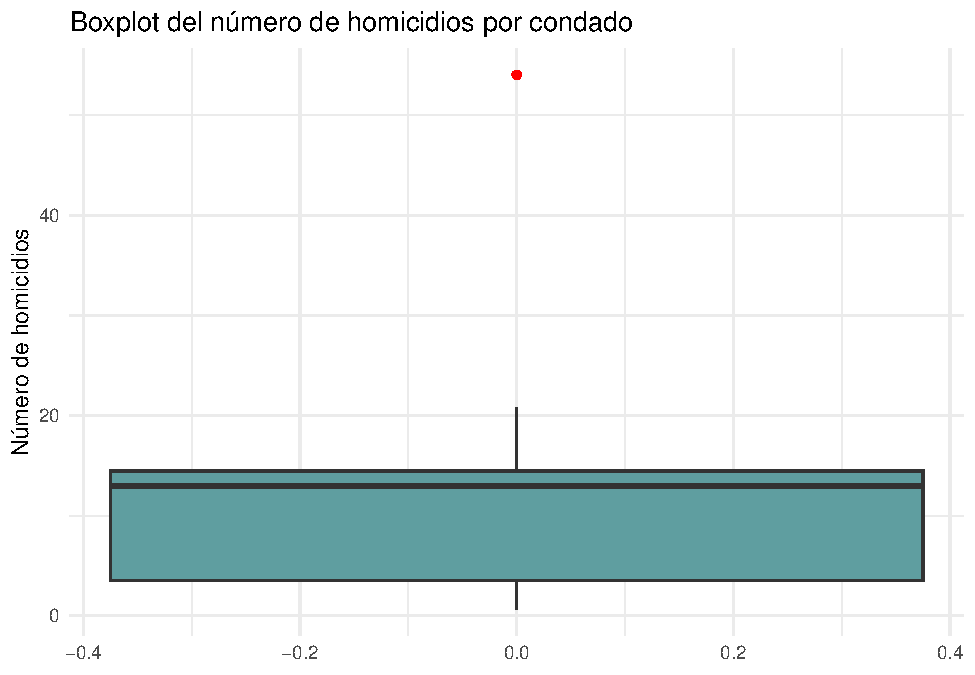
\includegraphics{Informe_P2_files/figure-latex/boxplot-homicidios-1.pdf}

\begin{Shaded}
\begin{Highlighting}[]
\FunctionTok{ggsave}\NormalTok{(}\StringTok{"../salida/boxplot\_homicidios.png"}\NormalTok{, }\AttributeTok{width =} \DecValTok{6}\NormalTok{, }\AttributeTok{height =} \DecValTok{4}\NormalTok{, }\AttributeTok{bg =} \StringTok{"white"}\NormalTok{)}
\end{Highlighting}
\end{Shaded}

\newpage

\subsection{Dispersión: ingreso vs esperanza de
vida}\label{dispersiuxf3n-ingreso-vs-esperanza-de-vida}

\begin{Shaded}
\begin{Highlighting}[]
\FunctionTok{ggplot}\NormalTok{(datos, }\FunctionTok{aes}\NormalTok{(}\AttributeTok{x =}\NormalTok{ avg\_income, }\AttributeTok{y =}\NormalTok{ life\_expectancy)) }\SpecialCharTok{+}
  \FunctionTok{geom\_point}\NormalTok{(}\AttributeTok{color =} \StringTok{"dodgerblue"}\NormalTok{, }\AttributeTok{size =} \DecValTok{3}\NormalTok{) }\SpecialCharTok{+}
  \FunctionTok{geom\_smooth}\NormalTok{(}\AttributeTok{method =} \StringTok{"lm"}\NormalTok{, }\AttributeTok{se =} \ConstantTok{FALSE}\NormalTok{, }\AttributeTok{color =} \StringTok{"grey"}\NormalTok{) }\SpecialCharTok{+}
  \FunctionTok{labs}\NormalTok{(}\AttributeTok{title =} \StringTok{"Relación entre ingreso medio y esperanza de vida"}\NormalTok{, }\AttributeTok{x =} \StringTok{"Ingreso medio"}\NormalTok{, }\AttributeTok{y =} \StringTok{"Esperanza de vida (años)"}\NormalTok{) }\SpecialCharTok{+}
  \FunctionTok{theme\_minimal}\NormalTok{()}
\end{Highlighting}
\end{Shaded}

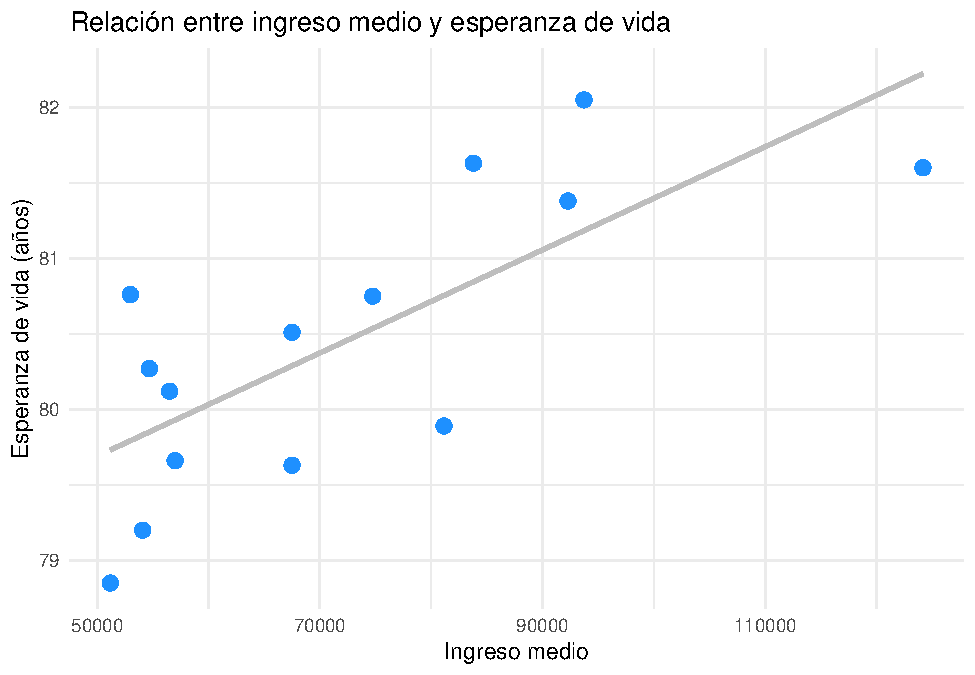
\includegraphics{Informe_P2_files/figure-latex/dispersion-1.pdf}

\begin{Shaded}
\begin{Highlighting}[]
\FunctionTok{ggsave}\NormalTok{(}\StringTok{"../salida/scatter\_income\_life\_expectancy.png"}\NormalTok{, }\AttributeTok{width =} \DecValTok{7}\NormalTok{, }\AttributeTok{height =} \DecValTok{5}\NormalTok{, }\AttributeTok{bg =} \StringTok{"white"}\NormalTok{)}
\end{Highlighting}
\end{Shaded}

\newpage

\subsection{Burbujas: ingreso, esperanza de vida y
salud}\label{burbujas-ingreso-esperanza-de-vida-y-salud}

\begin{Shaded}
\begin{Highlighting}[]
\FunctionTok{ggplot}\NormalTok{(datos, }\FunctionTok{aes}\NormalTok{(}\AttributeTok{x =}\NormalTok{ avg\_income, }\AttributeTok{y =}\NormalTok{ life\_expectancy, }\AttributeTok{size =}\NormalTok{ pop, }\AttributeTok{color =}\NormalTok{ poor\_health)) }\SpecialCharTok{+}
  \FunctionTok{geom\_point}\NormalTok{(}\AttributeTok{alpha =} \FloatTok{0.8}\NormalTok{) }\SpecialCharTok{+}
  \FunctionTok{scale\_size\_continuous}\NormalTok{(}\AttributeTok{range =} \FunctionTok{c}\NormalTok{(}\DecValTok{3}\NormalTok{, }\DecValTok{12}\NormalTok{)) }\SpecialCharTok{+}
  \FunctionTok{scale\_color\_gradient}\NormalTok{(}\AttributeTok{low =} \StringTok{"lightblue"}\NormalTok{, }\AttributeTok{high =} \StringTok{"darkred"}\NormalTok{) }\SpecialCharTok{+}
  \FunctionTok{labs}\NormalTok{(}
    \AttributeTok{title =} \StringTok{"Relación entre ingreso, salud, longevidad y población"}\NormalTok{,}
    \AttributeTok{x =} \StringTok{"Ingreso medio"}\NormalTok{,}
    \AttributeTok{y =} \StringTok{"Esperanza de vida"}\NormalTok{,}
    \AttributeTok{size =} \StringTok{"Población"}\NormalTok{,}
    \AttributeTok{color =} \StringTok{"Mala salud (\%)"}
\NormalTok{  ) }\SpecialCharTok{+}
  \FunctionTok{theme\_minimal}\NormalTok{()}
\end{Highlighting}
\end{Shaded}

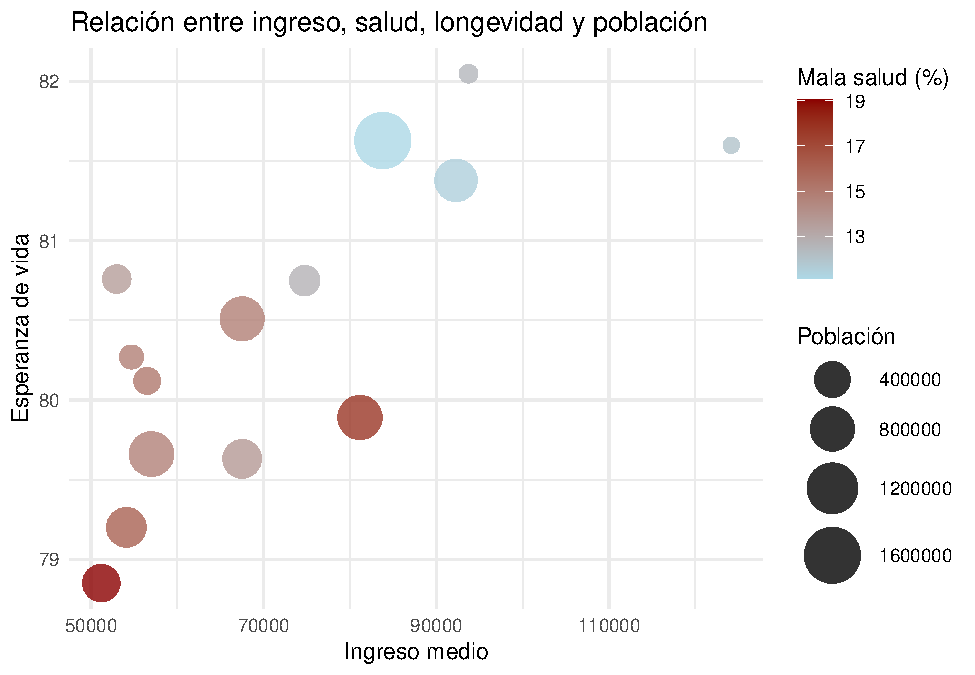
\includegraphics{Informe_P2_files/figure-latex/burbujas-1.pdf}

\begin{Shaded}
\begin{Highlighting}[]
\FunctionTok{ggsave}\NormalTok{(}\StringTok{"../salida/burbujas\_ingreso\_vida\_salud.png"}\NormalTok{, }\AttributeTok{width =} \DecValTok{8}\NormalTok{, }\AttributeTok{height =} \DecValTok{6}\NormalTok{, }\AttributeTok{bg =} \StringTok{"white"}\NormalTok{)}
\end{Highlighting}
\end{Shaded}

\newpage

\section{Conclusiones}\label{conclusiones}

\begin{itemize}
\tightlist
\item
  \textbf{Limpieza y preparación de los datos}: Se estandarizaron
  correctamente los nombres de las columnas y se imputaron los valores
  faltantes utilizando la media, dejando el conjunto de datos listo para
  el análisis.
\item
  \textbf{Estadísticas descriptivas}: Los resúmenes generados con
  \texttt{summary()} y \texttt{skim()} ofrecieron una visión detallada
  de las variables, permitiendo identificar tendencias generales, rangos
  y posibles valores extremos.
\item
  \textbf{Outliers}: Se detectaron valores atípicos significativos en
  variables como \texttt{suicides}, \texttt{homicides},
  \texttt{tasa\_homicidios}, \texttt{housing\_problems}, y proporciones
  de género. Estos fueron almacenados y analizados en una tabla final.
\item
  \textbf{Visualización de datos}:

  \begin{itemize}
  \tightlist
  \item
    El \textbf{histograma} y el \textbf{gráfico de densidad} mostraron
    una distribución sesgada del ingreso medio hacia la derecha.
  \item
    El \textbf{boxplot} de homicidios permitió identificar condados con
    tasas inusualmente altas.
  \item
    El \textbf{gráfico de dispersión} evidenció una relación positiva
    clara entre el ingreso medio y la esperanza de vida.
  \item
    El \textbf{gráfico de burbujas} integró ingreso, salud, esperanza de
    vida y población, mostrando patrones relevantes.
  \end{itemize}
\item
  \textbf{Análisis final}: Las visualizaciones y estadísticas respaldan
  la hipótesis de que mayores ingresos se asocian con mejores
  indicadores de salud y longevidad. La combinación de técnicas gráficas
  y análisis numérico facilitó la detección de patrones importantes en
  los datos.
\end{itemize}

\end{document}
